\documentclass[twoside,11pt]{article}
\usepackage{multirow}
\usepackage{jmlr2e}
\usepackage{lastpage}
\usepackage{amsmath}
\usepackage{booktabs}
\usepackage{appendix}

\jmlrheading{26}{2026}{1-\pageref{LastPage}}{11/11/26}{11/11/26}{25-0040}{Isaac Wilkey and Riley Smith}
\ShortHeadings{Linear, Feedforward, and Autoencoder Networks}{Wilkey and Smith}
\firstpageno{1}

\begin{document}

\title{Linear, Feedforward, and Autoencoder-Based Neural Networks for Classification and Regression}

\author{\name Isaac Wilkey \email isaac.wilkey@student.montana.edu\\
\addr Department of Computer Science \\
Montana State University \\
Bozeman, MT, USA
\AND
\name Riley Smith \email riley.smith13@student.montana.edu\\
\addr Department of Computer Science \\
Montana State University \\
Bozeman, MT, USA
}
\editor{Isaac Wilkey \& Riley Smith}

\maketitle

\begin{abstract}
TODO

\end{abstract}

\begin{keywords}neural networks, backpropagation, autoencoder, logistic regression, hyperparameter tuning $5 \times 2$ cross validation\end{keywords}

\section{Problem Statement and Hypotheses}
The goal of this project is to implement and analyze neural networks for classification and regression. A linear network maps inputs directly to outputs and can only model linear relationships. Hidden layers allow nonlinear modeling but add hyperparameters and a risk of overfitting. An autoencoder learns a compressed representation of the inputs without using labels. We implement a linear network, a feedforward network with two hidden layers, and a network whose first hidden layer is initialized from an autoencoder.

We test the following hypotheses using $5 \times 2$ cross validation \citep{alpaydin2020}:
\begin{enumerate}
    \item \textbf{H1:} The two-hidden-layer neural networks will perform better in terms of classification error/mean squared error than the linear networks on a majority of the six datasets.
    \item \textbf{H2:} The autoencoder-based networks will perform better in terms of classification error/mean squared error than the two-hidden-layer neural networks on a majority of the six datasets.
\end{enumerate}
H1 is falsified if the linear network has the lower classification error/mean squared error than the two-hidden-layer neural network on three or more data sets. H2 is falsified if the two-hidden-layer neural network has the lower classification error/mean squared error than the autoencoder-based network on three or more data sets.


\section{Experimental Approach and Project Design}
Our experimental pipeline consisted of data acquisition, preprocessing, model creation, tuning, and evaluation.

\subsection{Datasets}
We utilize six datasets from the UCI repository \citep{uci_repository}. Three are classification tasks and three are regression tasks. Table~\ref{tab:datasets} summarizes the datasets.

\begin{table}[h]
    \centering
    \begin{tabular}{llcc}
    \hline
    Dataset & Task & Instances & Features (num./cat.) \\
    \hline
    Breast Cancer     & Classification & 699  & 9 (9/0) \\
    Car Evaluation    & Classification & 1728 & 6 (0/6) \\
    House Votes       & Classification & 435  & 16 (0/16) \\
    Abalone           & Regression     & 4177 & 8 (7/1) \\
    Computer Hardware & Regression     & 209  & 6 (6/0) \\
    Forest Fires      & Regression     & 517  & 12 (10/2) \\
    \hline
    \end{tabular}
    \caption{Summary of the six datasets used in this assignment.}
    \label{tab:datasets}
\end{table}

\subsection{Preprocessing}
We apply the following preprocessing steps to the UCI datasets:
\begin{itemize}
    \item \textbf{Breast Cancer:} We replace missing values (marked with "?") with the mode of mode of that feature. We also drop the sample code number feature as it is a unique identifier. Finally, we apply z score normalization to all numerical features.
    \item \textbf{Car Evaluation:} We label encode all features to maintain their order as integers. We then apply z score normalization to all features.
    \item \textbf{House Votes:} We one hot encode all features.
    \item \textbf{Abalone:} We one hot encode the only categorical feature. We then apply z score normalization to all features.
    \item \textbf{Computer Hardware:} We drop the vendor name and model name features as unique identifiers. We also drop the erp feature as it is the dataset authors' own linear regression estimate of the target. We then apply z score normalization to all features.
    \item \textbf{Forest Fires:} We cyclic encode the month and day features. We then apply z score normalization to all features. Finally, we log transform the target.
\end{itemize}

\subsection{Evaluation Protocol}
To obtain a fair comparison between each model, we employ a $5 \times 2$ cross-validation framework. The data is split into two halves; we train on half and test on the other, then reverse the roles. This process is repeated five times with different random splits. We repeat this process for each model.

For classification we report the classification error, the fraction of test instances predicted incorrectly:
\begin{equation}
    \text{Classification Error} = \frac{1}{N}\sum_{t=1}^{N} \mathbf{1}\left[\hat{r}^t \neq r^t\right],
\end{equation}
and for regression we report the mean squared error,
\begin{equation}
    \text{MSE} = \frac{1}{N}\sum_{t=1}^{N} \left(r^t - \hat{r}^t\right)^2,
\end{equation}
where $N$ is the number of test instances.

\section{Algorithms Implemented}
TODO

\subsection{Logistic Regression}
Logistic regression is a linear network with no hidden layers. The $d$ input features connect directly to an output layer with one node per class. For $K$ classes, class $C_i$ has a weight vector $\mathbf{w}_i \in \mathbb{R}^{d}$ and a bias $w_{i0}$. For an input $\mathbf{x}$, the output for class $C_i$ is given by the softmax function:
\begin{equation}
    y_i = P(C_i|\mathbf{x}) = \frac{\exp\left[\mathbf{w}_i^{\top}\mathbf{x} + w_{i0}\right]}{\sum_{j=1}^{K}\exp\left[\mathbf{w}_j^{\top}\mathbf{x} + w_{j0}\right]}
\end{equation}
The predicted class is output with the largest $y_i$. The network minimizes the cross-entropy loss, which we average over a batch $B$ of instances:
\begin{equation}
    L = -\frac{1}{|B|}\sum_{t \in B}\sum_{i=1}^{K} r_i^t \log y_i^t
\end{equation}
For softmax combined with cross-entropy, the gradient simplifies to the difference between the labels and the outputs. This gives the following update for each class:
\begin{equation}
    \Delta\mathbf{w}_i = \frac{\eta}{|B|}\sum_{t \in B}(r_i^t - y_i^t)\,\mathbf{x}^t, \qquad
    \Delta w_{i0} = \frac{\eta}{|B|}\sum_{t \in B}(r_i^t - y_i^t)
\end{equation}
where $\eta$ is the learning rate. We train with mini-batch gradient descent. The weights are initialized from a normal distribution with mean $0$ and standard deviation $0.01$. The biases are initialized to zero. In each epoch, we shuffle the training set, divide it into batches, and update $\mathbf{w}_i \leftarrow \mathbf{w}_i + \Delta\mathbf{w}_i$ and $w_{i0} \leftarrow w_{i0} + \Delta w_{i0}$ after each batch for every class. We treat the learning rate, batch size, and number of epochs as tuned hyperparameters (Section~\ref{sec:tuning}).

\subsection{Linear Regression}
Linear regression is a linear network with no hidden layers. The $d$ input features connect to a single output node. The output node has a weight vector $\mathbf{w} \in \mathbb{R}^{d}$ and a bias $w_0$. For an input $\mathbf{x}$, the prediction is:
\begin{equation}
    y = \mathbf{w}^{\top}\mathbf{x} + w_0
\end{equation}
The network minimizes the squared error between the predictions and the targets, which we average over a batch $B$ of instances:
\begin{equation}
    L = \frac{1}{|B|}\sum_{t \in B}(r^t - y^t)^2
\end{equation}
We minimize this loss using gradient descent. This gives the following update:
\begin{equation}
    \Delta\mathbf{w} = \frac{\eta}{|B|}\sum_{t \in B}(r^t - y^t)\,\mathbf{x}^t, \qquad
    \Delta w_0 = \frac{\eta}{|B|}\sum_{t \in B}(r^t - y^t)
\end{equation}
where $\eta$ is the learning rate. We train with mini-batch gradient descent. The weights are initialized from a normal distribution with mean $0$ and standard deviation $0.01$. The bias is initialized to zero. In each epoch, we shuffle the training set, divide it into batches, and update $\mathbf{w} \leftarrow \mathbf{w} + \Delta\mathbf{w}$ and $w_{0} \leftarrow w_{0} + \Delta w_{0}$ after each batch. We treat the learning rate, batch size, and number of epochs as tuned hyperparameters (Section~\ref{sec:tuning}).

\subsection{Neural Network}
TODO

\subsection{Autoencoder}
TODO

\subsection{Autoencoder-Based Network}
TODO

\subsection{Hyperparameter Tuning}
\label{sec:tuning}
TODO


\section{Experimental Results}
We evaluate each model using $5 \times 2$ cross validation on each of the six datasets, as described in Section 2.3. We report classification error for the three classification datasets and mean squared error for the three regression datasets. Every value is the mean over the ten test folds.

\subsection{Classification}
Table~\ref{tab:classification-results} reports classification error for the three models on the three classification datasets, and Figure~\ref{fig:error} (left) shows the same comparison.

\begin{table}[h]
    \centering
    \begin{tabular}{lccc}
    \hline
    Dataset & Linear & Two-Hidden-Layer & Autoencoder-Based \\
    \hline
    Breast Cancer   & 0.0369 & 0.0326 & 0.0358 \\
    Car Evaluation  & 0.1702 & 0.0395 & 0.1593 \\
    House Votes     & 0.0402 & 0.0632 & 0.0385 \\
    \hline
    \end{tabular}
    \caption{Classification error ($5 \times 2$ CV mean) for the three models.}
    \label{tab:classification-results}
\end{table}

The two-hidden-layer network lowers the mean error relative to the linear network on Breast Cancer and Car Evaluation, by 11.7\% and 76.8\% respectively. On House Votes it raises the error by 57.2\%. The autoencoder-based network lowers the error relative to the linear network on all three data sets, by 3.0\% on Breast Cancer, 6.4\% on Car Evaluation, and 4.2\% on House Votes It is also the best model on House Votes.

\subsection{Regression}
Table~\ref{tab:regression-results} reports mean squared error for the three models on the three regression datasets, and Figure~\ref{fig:error} (right) shows the same comparison. Forest Fires errors are on the log scale of the transformed target described in Section 2.2.

\begin{table}[h]
\centering
\begin{tabular}{lccc}
\hline
Dataset & Linear & Two-Hidden-Layer & Autoencoder-Based \\
\hline
Abalone            & 0.4902      & 0.4392      & 0.4550 \\
Computer Hardware  & 0.2464      & 0.2790      & 0.2286 \\
Forest Fires       & 1.1589      & 1.0394      & 1.0387 \\
\hline
\end{tabular}
\caption{Mean squared error ($5 \times 2$ CV mean) for the three models.}
\label{tab:regression-results}
\end{table}

\begin{figure}[h]
    \centering
    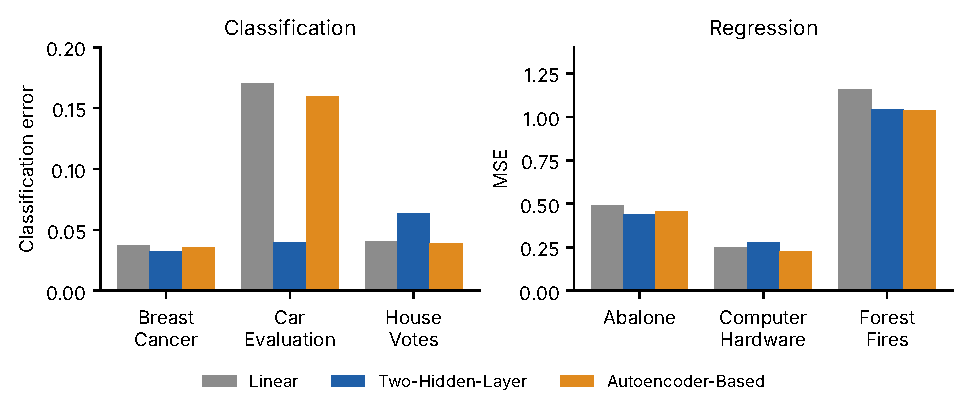
\includegraphics[width=\linewidth]{figures/results_figure.pdf}
    \caption{Test error for three models on the classification datasets (left) and regression datasets (right). Bars show the mean over the ten folds.}
    \label{fig:error}
\end{figure}

The two-hidden-layer network lowers the mean squared error relative to the linear network on Abalone and Forest Fires, by 10.4\% and 10.3\% respectively, but raises it by 13.2\% on Computer Hardware. The autoencoder-based network lowers the error on all three data sets, by 7.2\% on Abalone, 7.2\% on Computer Hardware, and 10.4\% on Forest Fires. It is the best model on Computer Hardware and Forest Fires. The two-hidden-layer network is the best on Abalone. 

\subsection{Linear Network Hyperparameters}
Table~\ref{tab:linear-tuning} reports the tuned hyperparamaters for the linear models for the six datasets.

\begin{table}[h]
    \centering
    \begin{tabular}{lccc}
    \hline
    Dataset & Learning Rate & Batch Size & Epochs \\
    \hline
    Breast Cancer      & 0.9809    & 26   & 950 \\
    Car Evaluation     & 0.6341   & 124 & 850 \\
    House Votes        & 0.5474    & 29    & 50 \\
    Abalone            & 0.0702  & 257 & 650 \\
    Computer Hardware  & 0.1545   & 8  & 200 \\
    Forest Fires       & 0.0661   & 41  & 300 \\
    \hline
    \end{tabular}
    \caption{Tuned learning rate, batch size, and epochs for the linear networksnetworks for the six datasets.}
    \label{tab:linear-tuning}
\end{table}

\subsection{Two-Hidden-Layer Network Hyperparameters}
Table~\ref{tab:hidden-tuning} reports the tuned hyperparamaters for the two-hidden-layer networks for the six datasets.

\begin{table}[h]
    \centering
    \begin{tabular}{lccccc}
    \hline
    Dataset & Learning Rate & Batch Size & Epochs & Hidden 1 & Hidden 2 \\
    \hline
    Breast Cancer      & 0.3086    & 27   & 50  & 15    & 15 \\
    Car Evaluation     & 0.3886   & 10 & 1000    & 11   & 3 \\
    House Votes        & 0.3042    & 28    & 50     & 28    & 15 \\
    Abalone            & 0.1538  & 45 & 550     & 19    & 5 \\
    Computer Hardware  & 0.2123   & 16  & 350   & 7     & 7 \\
    Forest Fires       & 0.0309   & 9  & 350    & 20    & 19 \\
    \hline
    \end{tabular}
    \caption{Tuned learning rate, batch size, epochs, number of nodes in the first hidden layer, and number of nodes in the second hidden layer for the two-hidden-layer networks for the six datasets.}
    \label{tab:hidden-tuning}
\end{table}

\subsection{Autoencoder-Based Network Hyperparameters}
Table~\ref{tab:autoencoder-tuning} reports the tuned hyperparamaters for the autoencoder-based networks for the six datasets.

\begin{table}[h]
    \centering
    \begin{tabular}{lccccc}
    \hline
    Dataset & Learning Rate & Batch Size & Epochs & Autoencoder & Hidden \\
    \hline
    Breast Cancer      & 0.6046    & 27   & 650  & 5    & 12 \\
    Car Evaluation     & 0.1545   & 12 & 950    & 5   & 8 \\
    House Votes        & 0.0702    & 25    & 650     & 32    & 18 \\
    Abalone            & 0.1570  & 21 & 950     & 9    & 15 \\
    Computer Hardware  & 0.1545   & 8  & 800   & 5     & 8 \\
    Forest Fires       & 0.0459   & 33  & 150    & 11    & 17 \\
    \hline
    \end{tabular}
    \caption{Tuned learning rate, batch size, epochs, number of nodes in the autoencoder layer, and number of nodes in the second hidden layer for the autoencoder-based networks for the six datasets.}
    \label{tab:autoencoder-tuning}
\end{table}

\section{Analysis and Discussion}
TODO

\subsection{Preprocessing}
TODO

\subsection{Hypotheses}
TODO

\subsection{Tuning}
TODO

\section{Conclusion}
TODO

\bibliography{references}

\newpage

\appendix
\section{Main Lessons Learned}
TODO

\section{Delineation of Work}
\begin{itemize}
    \item \textbf{Isaac Wilkey:} Responsible for the implementation of the core machine learning algorithms, specifically developing the decision tree growth logic using Gain Ratio for classification and Mean Squared Error for regression, as well as the reduced error pruning system. Additionally, I authored the Abstract, the Algorithms Implemented section, and the Conclusion of the final report.
    \item \textbf{Riley Smith:} Responsible for the implementation of the preprocessing and evaluation algorithms. In the report, I authored the Problem Statement and Hypothesis, Experimental Approach and Project Design, Experimental Results, and Analysis and Discussion sections. 
\end{itemize}

\end{document}